% Компіляція: lualatex -shell-escape main.tex
\documentclass[12pt,a4paper]{article}
\usepackage{fontspec,polyglossia}
\setdefaultlanguage{ukrainian}
\setmainfont{NewComputerModern10}
\setmonofont{Noto Sans Mono}[Scale=0.82]
\usepackage{amsmath,booktabs,caption,enumitem,float,fvextra,geometry,graphicx,hyperref,microtype,tikz,titlesec}
\usetikzlibrary{arrows.meta,positioning}
\geometry{left=2cm,right=2cm,top=2cm,bottom=2cm}
\setlength{\parindent}{1.25cm}\setlength{\parskip}{0pt}\linespread{1.0}
\setlength{\emergencystretch}{3em}
\captionsetup{font=small,labelfont=bf,labelsep=endash}
\titleformat{\section}{\normalfont\fontsize{14}{16}\selectfont\bfseries\centering}{\thesection.}{0.6em}{}
\titleformat{\subsection}{\normalfont\fontsize{12}{14}\selectfont\bfseries\centering}{\thesubsection.}{0.6em}{}
\begin{document}
\pagenumbering{gobble}
\begin{titlepage}
\begin{center}
\includegraphics[width=.7\textwidth]{../../../../../../templates/letterhead.png}\end{center}
\begin{center}\large Національний технічний університет України\\
«Київський політехнічний інститут імені Ігоря Сікорського»\\[1em]
Факультет інформатики та обчислювальної техніки\\Кафедра обчислювальної техніки\end{center}
\vfill
\begin{center}\textbf{\LARGE Технології Computer Vision}\\[2em]
\textbf{\Large Лабораторна робота №5}\\[.7em]
«Технології кластеризації та класифікації в Computer Vision»\end{center}
\vfill
\begin{flushright}\begin{minipage}{.48\textwidth}
Виконав: студент 3 курсу ФІОТ,\\групи ІО-41\\\textit{Давидчук А. М.}\\
Залікова книжка № 4106\\[1em]Перевірив: \textit{Баран Д. Р.}
\end{minipage}\end{flushright}
\vfill\begin{center}Київ --- 2026\end{center}
\end{titlepage}
\pagenumbering{arabic}

\section{Тема та мета роботи}
\noindent\textbf{Тема:} технології кластеризації та сегментації цифрових зображень.

\medskip
\noindent\textbf{Мета:} дослідити практичне застосування кластеризації цифрових зображень у задачах Computer Vision без використання методів глибинного навчання.

\section{Завдання роботи}
Для отримання максимальних 10 балів реалізовано дві групи вимог методички:
\begin{enumerate}[leftmargin=*]
\item удосконалити програмний компонент попередньої роботи, додавши кластеризацію та сегментацію двох знімків ДЗЗ;
\item кластеризувати не менше 10 знімків або фрагментів поверхні Землі за встановленими ознаками; спосіб кластеризації обрати самостійно, бажано без глибинного навчання.
\end{enumerate}
Використано два знімки кампусу КПІ з ЛР4 та 12 їхніх просторово різних фрагментів. Алгоритм $k$-means реалізовано власноруч засобами NumPy.

\section{Математична модель}
Кожен піксель подано ознаками
\begin{equation}x_i=[R_i,G_i,B_i,\lambda_x x_i/W,\lambda_y y_i/H]^T,\qquad \lambda_x=\lambda_y=0{,}22.\end{equation}
Кластеризація мінімізує суму квадратів відстаней до центрів:
\begin{equation}J=\sum_{j=1}^{K}\sum_{x_i\in C_j}\lVert x_i-\mu_j\rVert_2^2,\qquad
\mu_j=\frac1{|C_j|}\sum_{x_i\in C_j}x_i.\end{equation}
Для кластеризації фрагментів сформовано вектор із середніх та стандартних відхилень RGB, середніх модулів градієнтів $G_x,G_y$ і восьми інтервалів гістограми яскравості. Перед $k$-means ознаки стандартизовано:
\begin{equation}z_{ij}=\frac{x_{ij}-\bar x_j}{s_j+\varepsilon}.\end{equation}

\section{Архітектура рішення}
\begin{figure}[H]\centering
\begin{tikzpicture}[node distance=.7cm,block/.style={draw,rounded corners,align=center,minimum width=3cm,minimum height=.8cm,fill=blue!7},arrow/.style={-{Latex},thick}]
\node[block](a){Два знімки ДЗЗ};
\node[block,right=of a](b){RGB + координати};
\node[block,right=of b](c){Сегментація\\$k$-means, $K=6$};
\node[block,below=of c](d){12 фрагментів};
\node[block,left=of d](e){Статистичні та\\текстурні ознаки};
\node[block,left=of e](f){Кластери сцен\\$K=4$};
\draw[arrow](a)--(b)--(c)--(d)--(e)--(f);
\end{tikzpicture}
\caption{Блок-схема програмного рішення}
\end{figure}

\section{Результати}
\begin{figure}[H]\centering
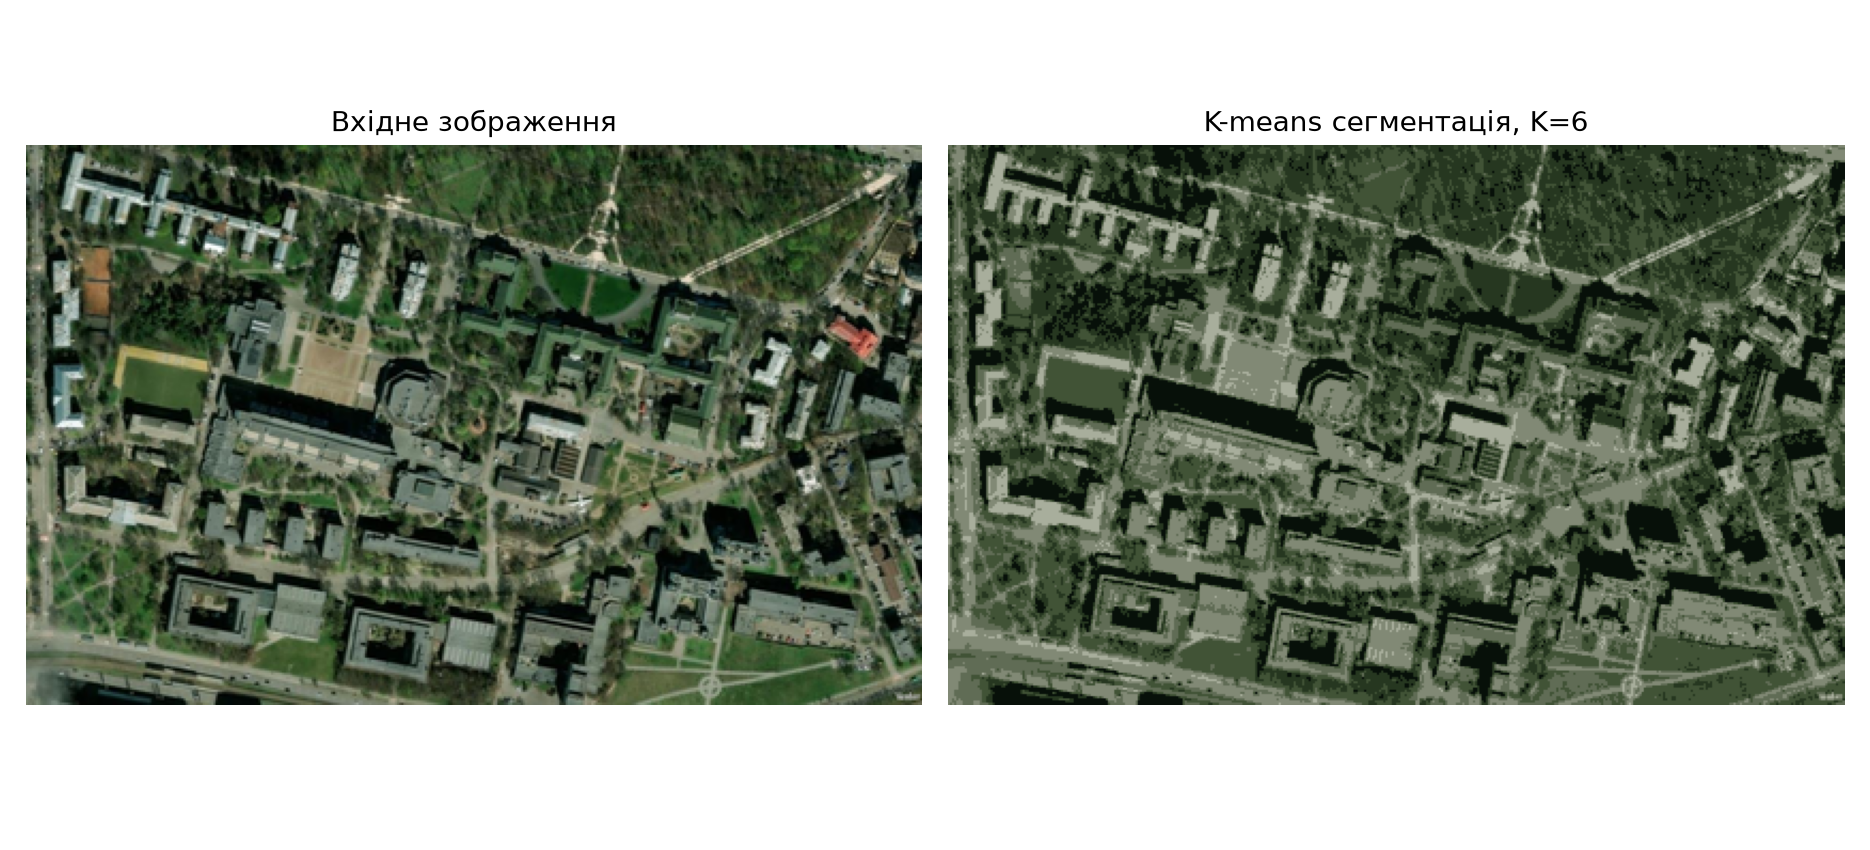
\includegraphics[width=.96\textwidth]{../results/segmentation_landsat.png}
\caption{Сегментація першого знімка методом $k$-means}
\end{figure}
\begin{figure}[H]\centering
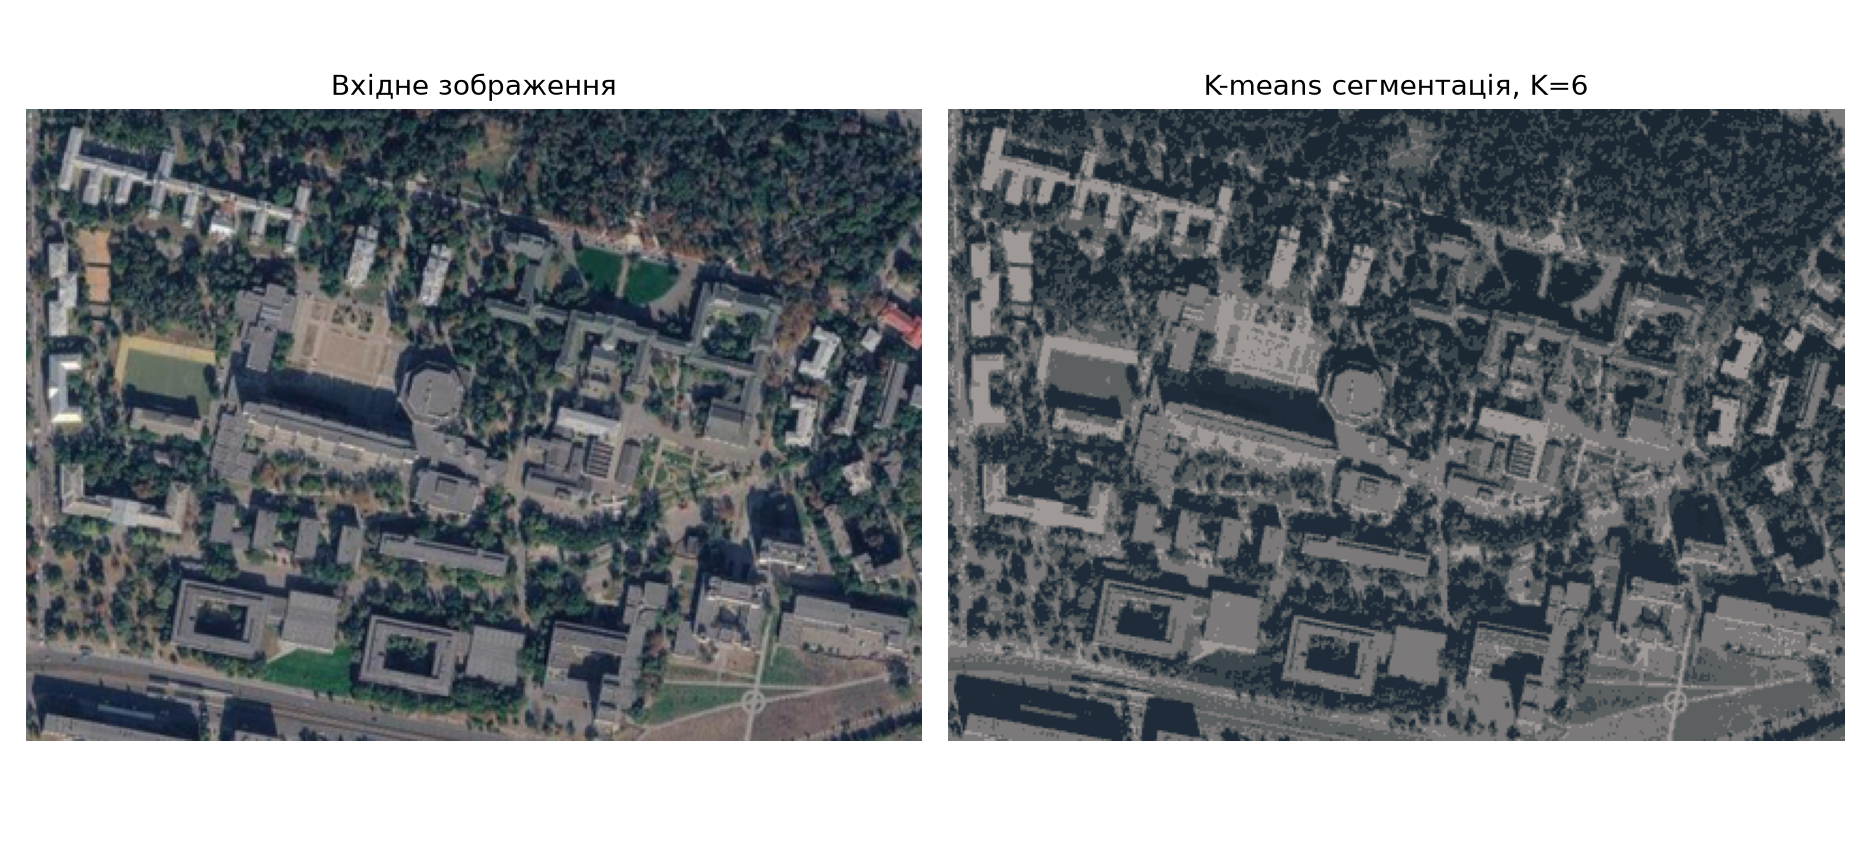
\includegraphics[width=.96\textwidth]{../results/segmentation_bing.png}
\caption{Сегментація другого знімка методом $k$-means}
\end{figure}
Алгоритм розділив пікселі на шість спектрально-просторових груп. Додавання нормованих координат не дає однаковим кольорам із віддалених частин кадру безумовно злитися в один сегмент.

\begin{figure}[H]\centering
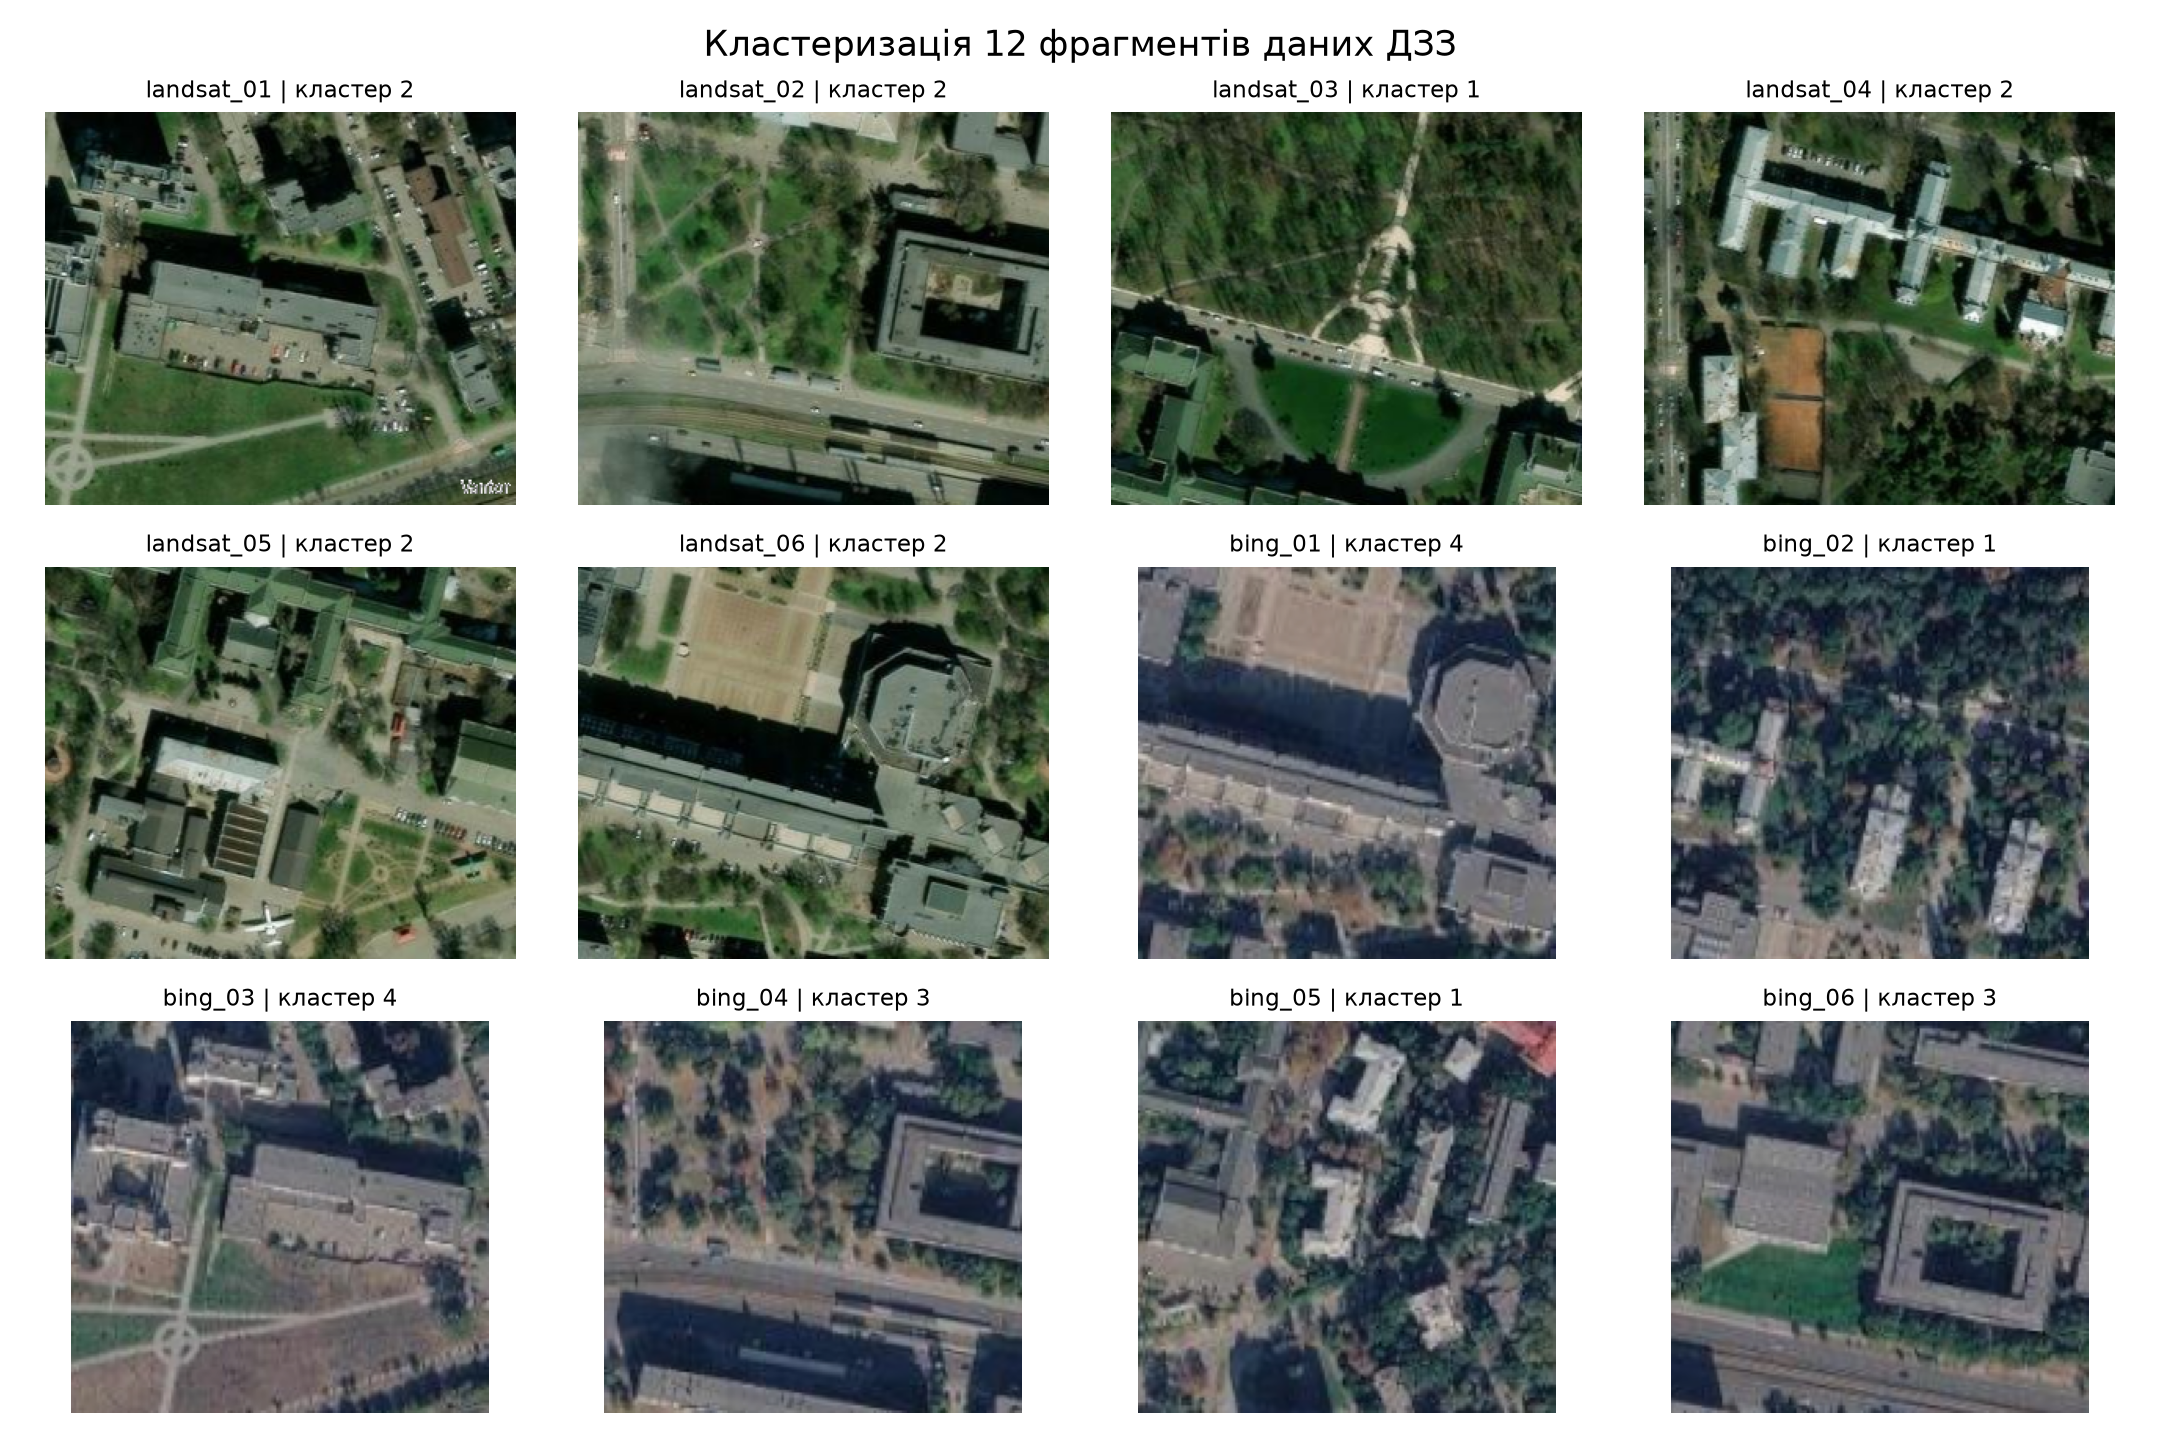
\includegraphics[width=.98\textwidth]{../results/patch_clusters.png}
\caption{Кластеризація 12 фрагментів поверхні Землі}
\end{figure}
\begin{table}[H]\centering\caption{Кількість фрагментів у кластерах}
\begin{tabular}{ccccc}\toprule Кластер&1&2&3&4\\\midrule Кількість&3&5&2&2\\\bottomrule\end{tabular}
\end{table}
Результат показує поділ не лише за джерелом знімка. Наприклад, фрагменти з переважанням рослинності потрапляють до спільної групи, а ділянки з великими дахами та щільною забудовою утворюють інші групи. Повний склад кластерів збережено у \texttt{clusters.csv}.

\section{Структура проєкту}
\begin{verbatim}
lab5/
|-- src/main.py
|-- results/*.png, clusters.csv
|-- requirements.txt
`-- docs/main.tex, main.pdf
\end{verbatim}

\section{Висновки}
Реалізовано обидві групи вимог ЛР5. Власний $k$-means сегментує два оперативні знімки, а другий етап кластеризує 12 фрагментів ДЗЗ за кольоровими, яскравісними та текстурними ознаками. Експеримент підтвердив, що класична кластеризація дає інтерпретований поділ без навчальної розмітки та нейромереж, але зміст кластерів визначається вибраними ознаками і параметром $K$.

\section{Лістинг програми}
\VerbatimInput[fontsize=\small,numbers=left,breaklines=true,frame=single]{../src/main.py}
\end{document}
